% Options for packages loaded elsewhere
\PassOptionsToPackage{unicode}{hyperref}
\PassOptionsToPackage{hyphens}{url}
\PassOptionsToPackage{dvipsnames,svgnames*,x11names*}{xcolor}
%
\documentclass[
  11,
]{article}
\usepackage{amsmath,amssymb}
\usepackage{lmodern}
\usepackage{ifxetex,ifluatex}
\ifnum 0\ifxetex 1\fi\ifluatex 1\fi=0 % if pdftex
  \usepackage[T1]{fontenc}
  \usepackage[utf8]{inputenc}
  \usepackage{textcomp} % provide euro and other symbols
\else % if luatex or xetex
  \usepackage{unicode-math}
  \defaultfontfeatures{Scale=MatchLowercase}
  \defaultfontfeatures[\rmfamily]{Ligatures=TeX,Scale=1}
\fi
% Use upquote if available, for straight quotes in verbatim environments
\IfFileExists{upquote.sty}{\usepackage{upquote}}{}
\IfFileExists{microtype.sty}{% use microtype if available
  \usepackage[]{microtype}
  \UseMicrotypeSet[protrusion]{basicmath} % disable protrusion for tt fonts
}{}
\makeatletter
\@ifundefined{KOMAClassName}{% if non-KOMA class
  \IfFileExists{parskip.sty}{%
    \usepackage{parskip}
  }{% else
    \setlength{\parindent}{0pt}
    \setlength{\parskip}{6pt plus 2pt minus 1pt}}
}{% if KOMA class
  \KOMAoptions{parskip=half}}
\makeatother
\usepackage{xcolor}
\IfFileExists{xurl.sty}{\usepackage{xurl}}{} % add URL line breaks if available
\IfFileExists{bookmark.sty}{\usepackage{bookmark}}{\usepackage{hyperref}}
\hypersetup{
  colorlinks=true,
  linkcolor=Maroon,
  filecolor=Maroon,
  citecolor=Blue,
  urlcolor=blue,
  pdfcreator={LaTeX via pandoc}}
\urlstyle{same} % disable monospaced font for URLs
\usepackage[margin=1in]{geometry}
\usepackage{longtable,booktabs,array}
\usepackage{calc} % for calculating minipage widths
% Correct order of tables after \paragraph or \subparagraph
\usepackage{etoolbox}
\makeatletter
\patchcmd\longtable{\par}{\if@noskipsec\mbox{}\fi\par}{}{}
\makeatother
% Allow footnotes in longtable head/foot
\IfFileExists{footnotehyper.sty}{\usepackage{footnotehyper}}{\usepackage{footnote}}
\makesavenoteenv{longtable}
\usepackage{graphicx}
\makeatletter
\def\maxwidth{\ifdim\Gin@nat@width>\linewidth\linewidth\else\Gin@nat@width\fi}
\def\maxheight{\ifdim\Gin@nat@height>\textheight\textheight\else\Gin@nat@height\fi}
\makeatother
% Scale images if necessary, so that they will not overflow the page
% margins by default, and it is still possible to overwrite the defaults
% using explicit options in \includegraphics[width, height, ...]{}
\setkeys{Gin}{width=\maxwidth,height=\maxheight,keepaspectratio}
% Set default figure placement to htbp
\makeatletter
\def\fps@figure{htbp}
\makeatother
\setlength{\emergencystretch}{3em} % prevent overfull lines
\providecommand{\tightlist}{%
  \setlength{\itemsep}{0pt}\setlength{\parskip}{0pt}}
\setcounter{secnumdepth}{5}
\usepackage{setspace}
\usepackage{hyperref}
\usepackage{graphicx}
\ifluatex
  \usepackage{selnolig}  % disable illegal ligatures
\fi
\newlength{\cslhangindent}
\setlength{\cslhangindent}{1.5em}
\newlength{\csllabelwidth}
\setlength{\csllabelwidth}{3em}
\newenvironment{CSLReferences}[2] % #1 hanging-ident, #2 entry spacing
 {% don't indent paragraphs
  \setlength{\parindent}{0pt}
  % turn on hanging indent if param 1 is 1
  \ifodd #1 \everypar{\setlength{\hangindent}{\cslhangindent}}\ignorespaces\fi
  % set entry spacing
  \ifnum #2 > 0
  \setlength{\parskip}{#2\baselineskip}
  \fi
 }%
 {}
\usepackage{calc}
\newcommand{\CSLBlock}[1]{#1\hfill\break}
\newcommand{\CSLLeftMargin}[1]{\parbox[t]{\csllabelwidth}{#1}}
\newcommand{\CSLRightInline}[1]{\parbox[t]{\linewidth - \csllabelwidth}{#1}\break}
\newcommand{\CSLIndent}[1]{\hspace{\cslhangindent}#1}

\author{}
\date{\vspace{-2.5em}}

\begin{document}

%%% .rmd + .sty setup borrowed from: https://github.com/oganm/ThesisProposal

\onehalfspacing
\pagenumbering{gobble}

%\begin{titlepage}
\begin{center}
\huge{\textbf{Efficacy of the radial tour and application to extend interpretability of black-box models when coupled with local explanations}}\\
\vspace*{1\baselineskip}
\Large{\textbf{Pre-submission review --- September 2021}}\\
%\vspace*{1\baselineskip}
\LARGE{Nicholas Spyrison, B.Sc}\\
\vspace*{1\baselineskip}

\LARGE{Monash University}\\
\Large{Faculty of Information Technology}\\
\Large{Department of Human-Centred Computing}\\
\vspace*{1\baselineskip}
\includegraphics[height = 3.5cm]{./figures/crest.jpg}\\
\vspace*{1\baselineskip}

\Large{\textbf{Thesis Supervisors}}\\
Prof. Kimbal Marriott\\
Prof. Dianne Cook\\
\vspace*{1\baselineskip}
\Large{\textbf{Committee Members}}\\
Dr. Maxime Cordiel\\
Dr. Shirui Pan\\
\vspace*{1\baselineskip}
\Large{\textbf{Chair}}\\
Assoc. Prof. Bernhard Jenny\\
\end{center}
% \end{titlepage}

\doublespacing

%\hypersetup{linkcolor = blue}
\newpage
\pagenumbering{roman}
\addcontentsline{toc}{section}{\contentsname}

\newpage

%% list of figures have to be added manually to table of contents
% \listoffigures 
% 
% \newpage
% \listoftables

\doublespacing

\newpage
\pagenumbering{arabic}
\hypersetup{linkcolor = blue}

{
\hypersetup{linkcolor=}
\setcounter{tocdepth}{2}
\tableofcontents
}
\hypertarget{sec:intro}{%
\section{Introduction}\label{sec:intro}}

The thesis of this work is central to multivariate data visualization. More specifically, we focus on the class of many linear projections are viewed near-continuously through small changes to the projection basis known as data visualization \emph{tours} Lee et al. (2021).

There are many variants of tours. We focus on one branch, \emph{manual tours} Spyrison and Dianne Cook (2020), that allows for user interaction by selecting one variable and specifying how to change its contribution to the current projection. By controlling the contribution of a single variable, a user can explore its sensitivity to the structure of the projection and identify which variables are ultimately most important to the structure in question. The work addressing the first research objective clarified the rationale for doing so and implements a free, open-source \texttt{R} package for applying the manual tour.

Next, we substantiated the efficacy of manual tours as compared with discrete combinations of principal components (Pearson 1901) and the \emph{grand tour}(Asimov 1985). We do so with an \(N=108\) within-participant user study, where all participants use each of these visual factors. This is performed over balanced trials across the other experimental factors: location, shape, and dimension of the data. This addresses the second research objective.

In our latest work, we want to see if we can apply the manual tour to aid the interpretability of complex, black-box models. One recent branch in explainable artificial intelligence (XAI, Adadi and Berrada (2018), Arrieta et al. (2020)) is the use of local explanations or attribution of the variables for one observation of an agnostic black-box model. One local explanation is the SHAP values (Lundberg and Lee 2017, EMA?). We use these SHAP values as a 1D basis and perform manual tours to explore how the SHAP values behave differently for misclassified and class-corrupted observations against neighboring correctly classified observations. This work corresponds to the third research objective

\hypertarget{motivation}{%
\section{Motivation}\label{motivation}}

The term exploratory data analysis (EDA) was coined by Tukey (1977), who leaves it as an intentionally broad term that encompasses the initial summarization and visualization of a data set, before a hypothesis to test has been formulated. This is a critical first step for understanding and becoming familiar with data and validating model assumptions. It may be tempting to review a series of summary statistics to check model assumptions. However, there are known datasets where the same summary statistics miss glaringly obvious visual patterns (Anscombe 1973; Matejka and Fitzmaurice 2017). It is easy to look at the wrong, or incomplete set of statistics needed to validate assumptions. Data visualization is crucial in EDA, it \emph{forces} you to see details and peculiarities of the data which are opaque to numeric summarization, or more nefariously, obscure their true values. Data visualization does and must remain a primary component of data analysis and model validation.

While static documents are the norm, there are sizable benefits of user interaction. Interactive data visualization shift the locus of control back to the user, inviting them to explore and interact with the data, and offers a compact way to explore a wider range of dimensions, questions, and keep the curiosity and the interest of the user.

With the emerging field of XAI, the constant tension between the interpretability of a model and its predictive power is receiving more attention. Linear models are the champions of interpretability with modest accuracy while increasing complex models improve accuracy but they can scarcely be interpreted even by experienced practitioners. One way to gain insight into a model is to focus on the local vicinity of one observation, and explain the variable weighting around that location, in an agnostic non-linear model. We call this observation level variable weights a \emph{local explanation}. There are various such local explanations, many are tied to specific classes of models, while others are model-agnostic.

We know that data visualization is important in EDA and assumption validation. User interaction allows us to explore widely and quickly while allowing us to explore ideas as they arise. These 2 elements were used to answer the first RO. Their efficacy was supported in response to the second RO. In this work, we apply tours in tandem with local explanations to extend the interpretability of black-box models, RO\#3.

\hypertarget{research-objectives}{%
\section{Research objectives}\label{research-objectives}}

The overall question of interest is:

\textbf{Can the geodesic interpolator with user interaction help analysts understand linear projections, and explore the sensitivity of structure in the projection to the variables contributing to the projection?}

Which is further divided into these more specific objectives:

\begin{enumerate}
\def\labelenumi{\arabic{enumi}.}
\item
  \textbf{How do we define user interaction for the geodesic interpolator to add and remove variables smoothly from a 2D linear projection of data?}\\
  Cook and Buja (1997) described an algorithm for manually controlling a tour, to rotate a variable into and out of a 2D projection. This algorithm provides the start to a human-controlled geodesic interpolator (GI). The work(Spyrison and Dianne Cook 2020) was adapted so that the user has more control of the interpolation. The user can set the full range of the contribution from \([-1, 1]\), and output to a device that allows the user to reproduce motions and animate or rock the rotation backward and forwards. These fine-tuned controls provide a better tool for sensitivity analysis.
\item
  \textbf{Do analysts understand the relationship between variables and structure in a 2D linear projection better when the geodesic interpolator is available?}\\
  We performed an \(N=108\), within-participant user study comparing accuracy and time with the primary factor as the type of data visualization. Each participant performed 2 evaluations with either discrete PCA, grand tour, or radial manual tour. We find strong evidence that the radial tour increases accuracy. We also show the effects from the other experimental factors of location, shape data dimensionality, and the random effects from the data and that of the participants.
\item
  \textbf{Can the geodesic interpolator be used in conjunction with the local explanation, SHAP, to improve the interpretability of black-box models?}\\
  The tension from the trade-off between accuracy and interpretability of black-box models is rising. Below we use SHAP to extract local explanations from a random forest model and use those SHAP values as a projection basis to perform manual tours. We add class-corrupted observations and explore how the model and SHAP values react.
\end{enumerate}

\hypertarget{methodology}{%
\section{Methodology}\label{methodology}}

The research corresponding with RO \#1 entails \emph{algorithm design} adapting the algorithm from Cook and Buja (1997). This allows for interactive control of 2D projections and serves as a foundation for the remaining work to follow.

To address RO \#2, a controlled \emph{experimental study} has explored the efficacy of interactive radial tours as compared with 2 benchmark methods: Principal Component Analysis (PCA, Pearson (1901)) and the grand tour(Asimov 1985). This was a within-participant user study where each participant experienced each visual. Trials were balanced across 3 other experimental factors: location of the signal, the shape of the cluster distributions, and the dimensionality of the data.

The research for RO \#3 involves \emph{fundamental visualization design}. We know that the SAHP value is a local explanation for one observation. This SHAP value will also serve as the 1D basis for the manual tour. While using SHAP as a projection basis is novel it is not particularly insightful by itself. We provide tracking marks on the tour as well as showing the within-class distributions of the SHAP components as parallel coordinate marks on the basis. We also offer a global view and quantitative analysis evaluating the sensitivity of the SHAP-space relative to the sensitivity of the original data space.

\hypertarget{work-since-the-mid-candidature-review}{%
\section{Work since the mid-candidature review}\label{work-since-the-mid-candidature-review}}

In the candidature confirmation review, we discussed the implementation of the \emph{geodesic interpolator} with user interaction (for RO \#1) which resulted in the open-source R package, \texttt{spinifex} available on CRAN and its subsequent publication (Spyrison and Dianne Cook 2020).

At the mid-candidature review, we discussed the experimental design of the user study to substantiate the efficacy of the radial tour as compared with PCA (discrete with user interaction), and the grand tour (continuous without user interaction). Below we briefly report our findings supporting RO\#2 before discussing the work addressing RO\#3.

\hypertarget{sec:expStudy}{%
\subsection{Experimental study}\label{sec:expStudy}}

The \(N=108\) within-participant user study collected 6 trials from each participant (648 total), with 2 trials of each of visuals: PCA, grand tour, and radial tour. Three further factors: location, shape, and data dimensionality were also evenly evaluated for a comparison with the effect of controlling the visuals. Participants were crowd-sourced from \texttt{prolific.co}, requiring that had completed an undergraduate degree and were compensated for their time at \pounds 7.50 per hour. Participants were tasked with identifying any and all variables contributing more than \(1/p\) to the separation of clusters.

\begin{figure}

{\centering 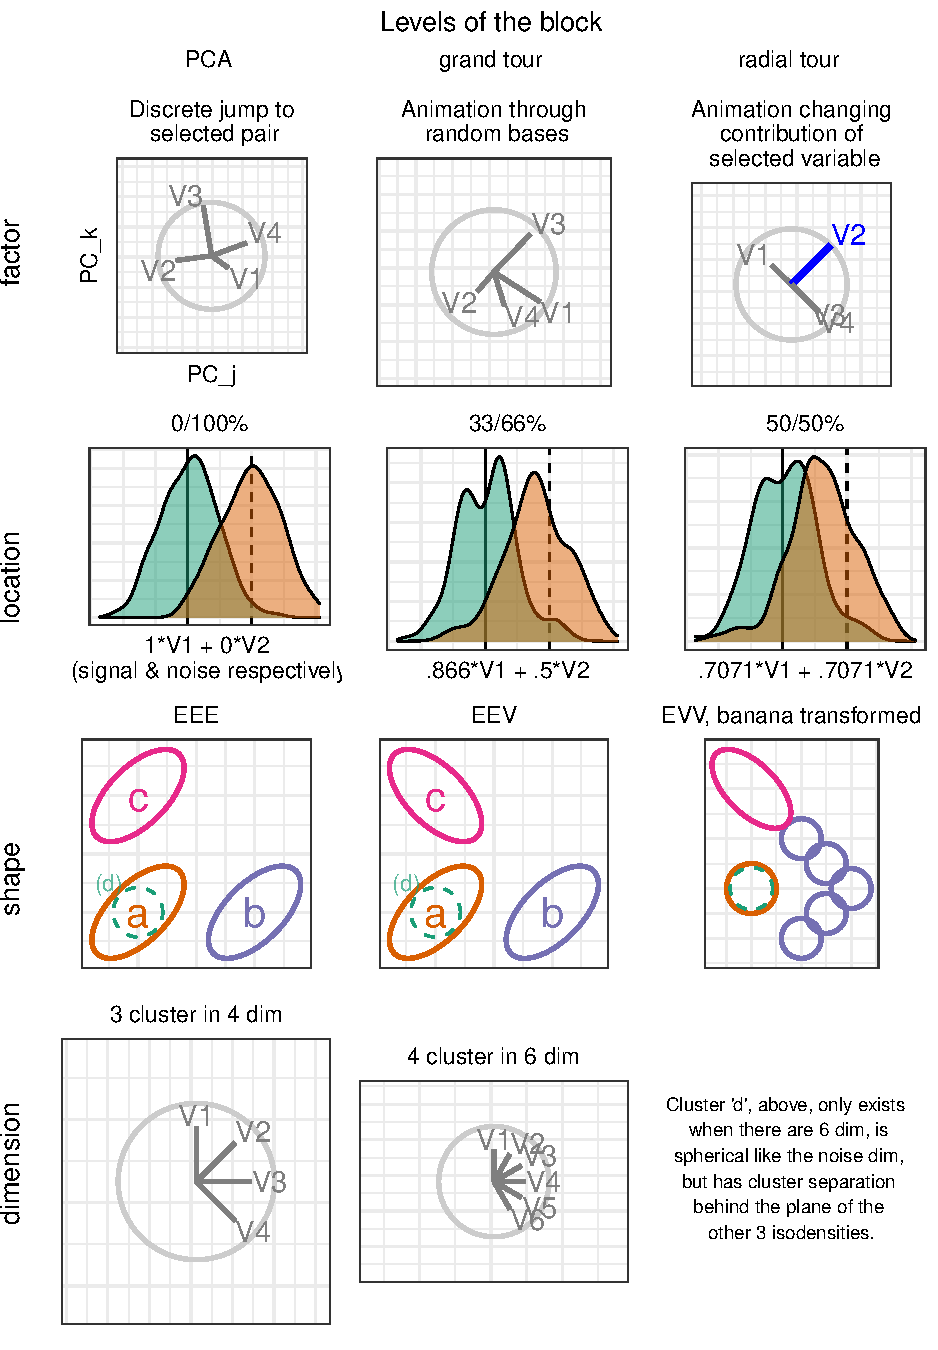
\includegraphics[width=0.9\linewidth,]{figures/study_exp_factors} 

}

\caption{The experimental factors of the study. Visualization is the primary factor of interest. The other factors extend the scope this problem is tested under.}\label{fig:studyExpFactors}
\end{figure}

In summary, we use a mixed regression model, to regress accuracy using the factors above as main effects, and use the participant and data simulations as random effects. The random effect capture the variation of the participant's skill and variation of difficulty due to the sampling of the data. Several models of increasing complexity were fit, and based on the model metrics select on the following model to explore the coefficient estimates of in detail.

\[
\begin{array}{ll}
&\widehat{Y} = \mu + \alpha_i * \beta_j + \textbf{Z} + \textbf{W} + \epsilon \\
\text{where } &\mu \text{ is the intercept of the model including the mean of random effect} \\
&\epsilon   \sim \mathcal{N}(0,~\sigma), \text{ the error of the model} \\
&\textbf{Z} \sim \mathcal{N}(0,~\tau), \text{ the random effect of participant} \\
&\textbf{W} \sim \mathcal{N}(0,~\upsilon), \text{ the random effect of simulation} \\
&\alpha_i \text{, fixed term for factor}~|~i\in (\text{pca, grand, radial}) \\
&\beta_j  \text{, fixed term for location}~|~j\in (\text{0\_1, 33\_66, 50\_50}) \text{ \% noise/signal mixing} \\
&\gamma_k \text{, fixed term for shape}~|~k\in (\text{EEE, EEV, EVV banana}) \text{ model shapes} \\
&\delta_l \text{, fixed term for dimension}~|~l\in (\text{4 variables \& 3 cluster, 6 variables \& 4 clusters}) \\
\end{array}
\]

\begin{figure}

{\centering 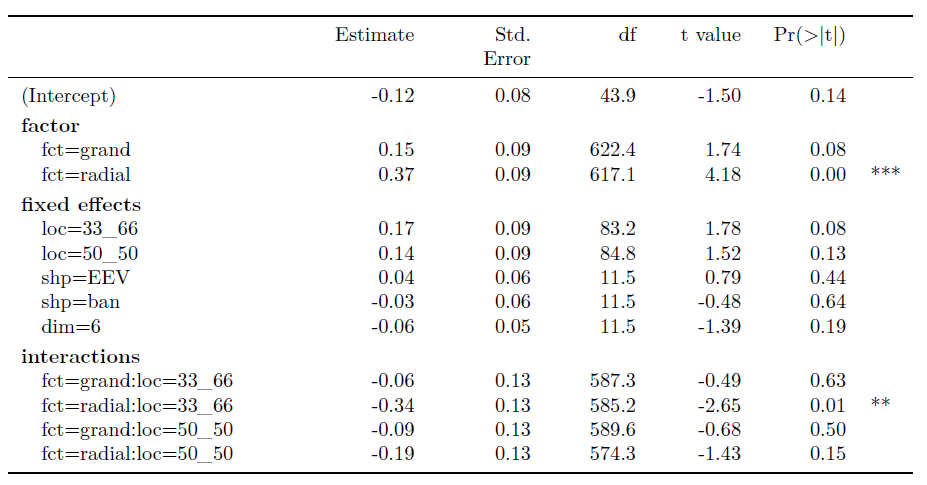
\includegraphics[width=1\linewidth,]{figures/spinifex_study_y1_results} 

}

\caption{Model coefficients regressing against our accuracy measure. We have strong evidence supporting a relatively large increase in accuracy with the radial tour.}\label{fig:studyResults}
\end{figure}

While radial tour is the new visualization, it is surprising that it is the only marginal term that is significant. Not only does it enjoy the most support, but it also has the largest coefficient estimates as well. Interestingly, the single significant interaction, radial, and location = 33/66\% has a large \emph{negative} coefficient, almost completely negating the gains from using radial when a signal and noise variable are mixed at that ratio. It is worth iterating that location, dimension, grand tour, and the intercept do have some evidence of having an effect.

A more in-depth description and discussion of this user study is attached as appendix A, a draft version of the paper, we intend to submit to the Journal of Data Science, Statistics, and Visualization. We also use the the same mixed regression model to predict log response time where the grand tour has the fastest responses, presumably due to the lack of interaction.

\hypertarget{extending-the-interpretation-of-black-box-models-with-the-use-of-interactive-continuous-linear-projections}{%
\subsection{Extending the interpretation of black-box models with the use of interactive continuous linear projections}\label{extending-the-interpretation-of-black-box-models-with-the-use-of-interactive-continuous-linear-projections}}

Local explanations describe the linear variable weights in the vicinity of an observation for a given model. For a highly-non linear space, the weightings of the variables will change more quickly in some areas than others. Local explanations are point-measurements of these weights that reveal how important each variable is to model at that particular location. There are several \emph{model-agnostic} local explanations such as LIME(Ribeiro, Singh, and Guestrin 2016), and SHAP(Lundberg and Lee 2017). In practice, any model and compatible local explanation can be used, however, we will be discussing and applying SHAP to a random forest model below.

\hypertarget{shap-values-local-variable-weights-and-additive-prediction-explanations.}{%
\subsubsection{SHAP values; local variable weights and additive prediction explanations.}\label{shap-values-local-variable-weights-and-additive-prediction-explanations.}}

To introduce the idea of SHAP values, consider FIFA soccer data(Leone 2020). We use 5000 player-observations of 9 aggregate skill measures to predict that player's wages. We use SHAP to observe how the skill attribution changes in the vicinity of players of different fielding positions. The intuition is that a model should change the weighting of the variables to more accurately predict the wages of the different positions' wages based solely on the values of explanatory skills and despite not explicitly knowing the fielding position.

We have trained a random forest model and wish to further explore the weightings of this non-linear model. Following the work in Biecek and Burzykowski (2021) we can similarly extract SHAP values, highlighting that different skills are valued differently across player positions within the model. We also show ``break down'' profiles, that is additive prediction explanations, how much of each player's predicted wages is added by each of the skill evaluations. The figure below takes a look at the SHAP and break down profiles of a star offensive and defensive player.

\begin{figure}

{\centering 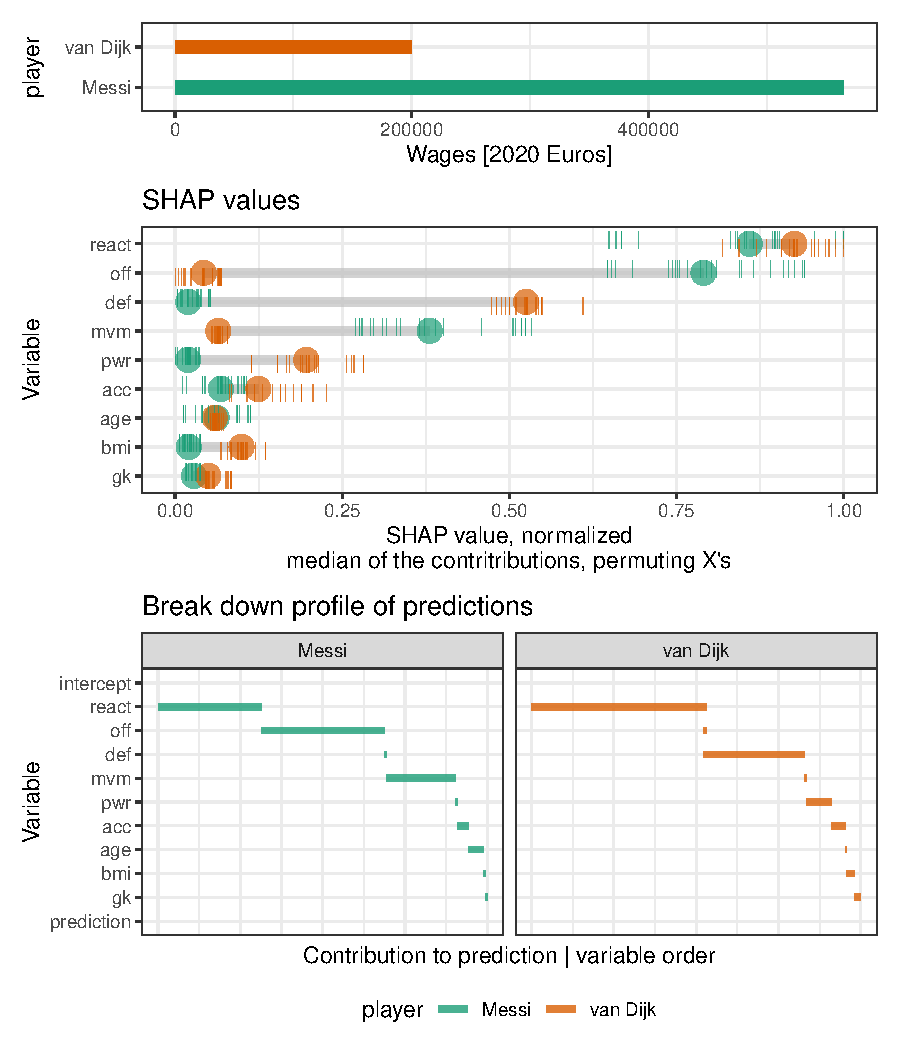
\includegraphics[width=1\linewidth]{figures/cheem_fifa_messi_dijk} 

}

\caption{SHAP values and prediction explanations of an offensive player (Messi, top) and a defensive player (van Dijk). SHAP values show a change in weights at the location of each player. Break down profiles show one order-sensitive explanation for the prediction of that observation.}\label{fig:cheemShapBd}
\end{figure}

\hypertarget{trees-of-cheem}{%
\subsubsection{Trees of Cheem}\label{trees-of-cheem}}

Above, we highlight the differing weights across 2 different fielder positions within the same model. It is hard to see where this fits in the full context of the other observations. Below we create a global (all observation) view by approximating the data- and SHAP-spaces in 2d with their first 2 principal components.

To illustrate this we take a look at much simpler data; a simulation of 3 spherical clusters on the vertices of a triangle. The difference between the clusters is contained in the first 2 dimensions with another 2 noise dimensions distributed as unit normal. After extracting all observation's SHAP values, forming a SHAP \emph{matrix}, of the original dimensionality, \((n~\times~p)\). We want to show a global view of the SHAP matrix and show how it and its sensitivity differ from that of the original data.

We approximate the data and SHAP spaces as the first 2 principal components. We facilitate exploration and interaction by adding a hovering tooltip displaying row number and class (actual \& predicted) with linked brushing highlighting selected points and displaying their data tabularly below the plot.

\begin{figure}

{\centering 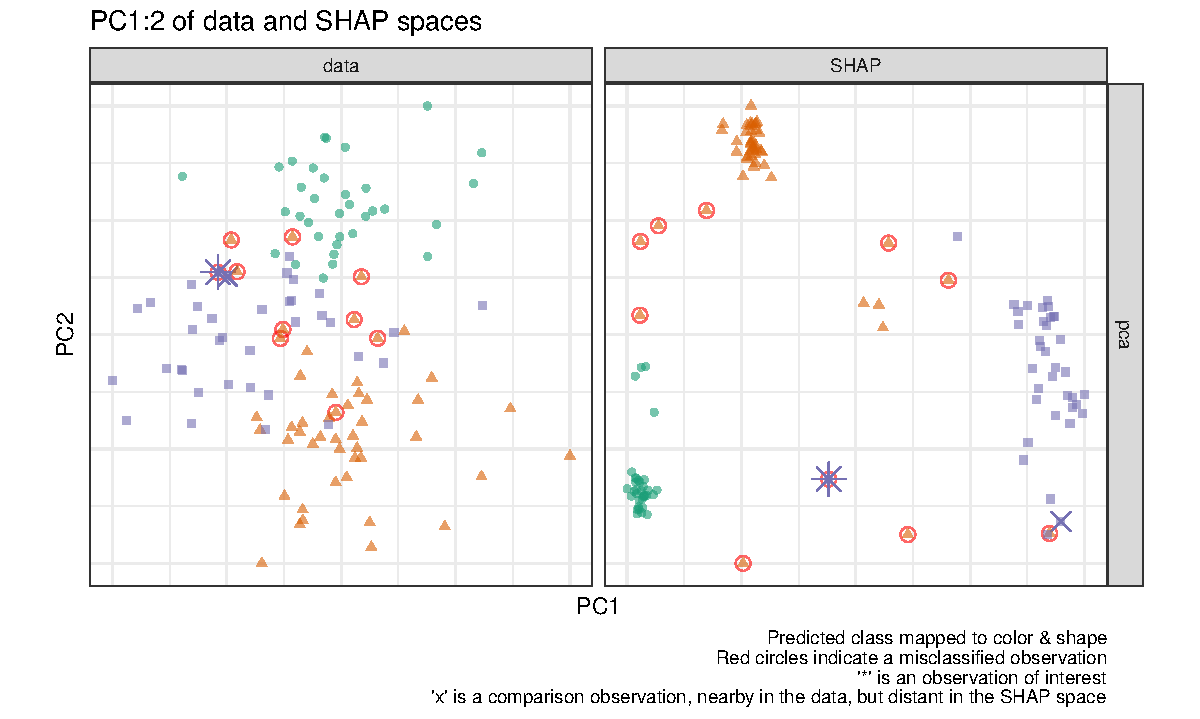
\includegraphics[width=1\linewidth]{figures/cheem_pca} 

}

\caption{Data and SHAP spaces (top and bottom respectively) of simulated data. The points are colored and shaped according to their predicted class, misclassified points are identified with a red circle. A target observation '*' is shown in comparison with nearby observation 'x'. These same 2 points are tracked in the proceeding tour.}\label{fig:cheemPca}
\end{figure}

Note that the bulk of the correctly classified points are clustered in relatively small areas. This means that the distribution of their SHAP values are quite similar; the model is selecting very tight variable weightings to explain the predicted class of each observation. Conversely, misclassified points tend to lie in between 2 clusters of correctly classified points. Using the interactive brushing and hover tool tips we confirm that these points lie between the actual and predicted classes.

Given the global view above we want to look at the local weightings of primary and comparison points (shown as '*/x' above and dashed/dotted lines below). In this case, the primary observation is misclassified while the comparison point is a correctly classified nearby point. These 2 points that are classified differently, but otherwise have very similar values in the explanatory variables, lie quite far apart in SHAP space.

Now we have the global context and an idea of the sensitivity of the SHAP spaces. To further explore an agnostic local explanation by exploring the structure created by the SHAP values of a particular observation. That is, it will be the projection that best puts this observation with its \emph{predicted class} and separate from the others. Consider the selected observation labeled as a star/asterisk above. Its normalized SHAP value will become the starting 1D basis to perform a radial tour exploring the structure. By default, the variable with the largest contribution is selected to be rotated fully into and out of projection. The location of the '*' and `x' observations are shown as the dashed and fainter, dotted lines respectively on the tour. Their current and initial (more faint, stationary) locations are highlighted throughout the tour.

\begin{figure}

{\centering 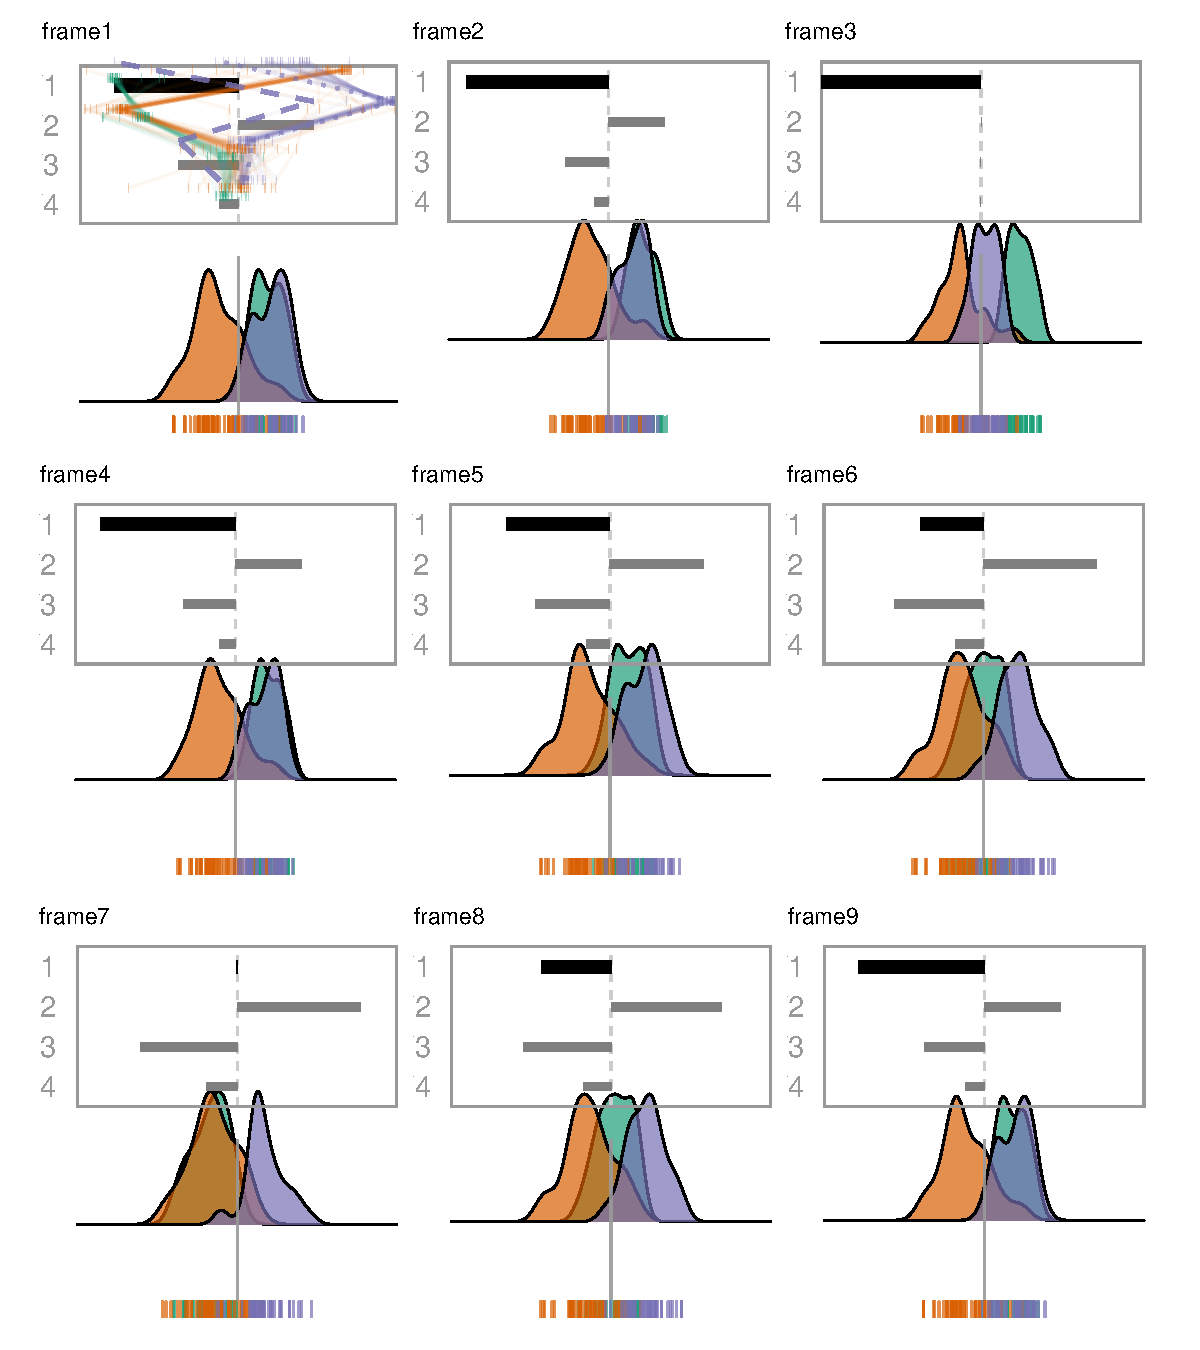
\includegraphics[width=1\linewidth]{figures/cheem_manualtour} 

}

\caption{The first frame of the radial tour. The SHAP values of the selected observation set the initial basis, shown as the grey and black bars on top. Within class distributions of the SHAP values are shown as parallel coordinate plots above each variable contribution. The class densities and observation positions of the 1D projection are shown on the bottom. The tour animates over small changes in the basis (top bars) as the variable with the largest contribution (weight) is rotated to have a full contribution, zero contribution, and then back to the initial contribution. A light grey line shows zero on the projection, with the dashed and dotted lines correspond to the position of primary and comparison observations ('*/x' in the preceding figure)}\label{fig:cheemTour}
\end{figure}

The application is in progress maturing and will be shown to experts for comment. This work is being written up to be submitted to the WHY-21 workshop, part of the NeurIPS 2021 Conference.

\hypertarget{discussion}{%
\subsubsection{Discussion}\label{discussion}}

We have used radial tours to improve the interpretability of black-box models by exploring the structure and distributions of the local explanations. It is important to note that this is independent of the quality of the model or even the quality of the explanation. Indeed the very term explanation feels like a bit of a misnomer as it seems to imply reason or validity, rather I prefer to think of it as local variable weightings of the model.

Keeping in mind the real-world application is particularly important. Finding methods to better interpret black-box models is an important challenge as corporations and nation-states increasingly use complex models to classify and predict their customers and citizens. Being able to glean insight into a models weights and how they differ for misclassified observations is extremely important for building and challenging models as we attempt to build a just world of tomorrow.

\hypertarget{proposed-thesis-structure-program-requirement}{%
\section{Proposed thesis structure \& program requirement}\label{proposed-thesis-structure-program-requirement}}

This is my assessment of the completion of the thesis research thus far:

\begin{itemize}
\tightlist
\item
  Introduction -- 60\%
\item
  Literature review -- 80\%
\item
  (RO \#1) GI \& manual tours -- 90\%
\item
  (RO \#2) manual tour efficacy user study -- 80\%
\item
  (RO \#3) manual tour interpretability, XAI -- 70\%
\item
  Discussion -- 50\%
\item
  Conclusion -- 30\%
\end{itemize}

The other requirements for this program are complete.

Figure \ref{fig:timeline} illustrates the purposed timeline for this research.

\begin{figure}

{\centering 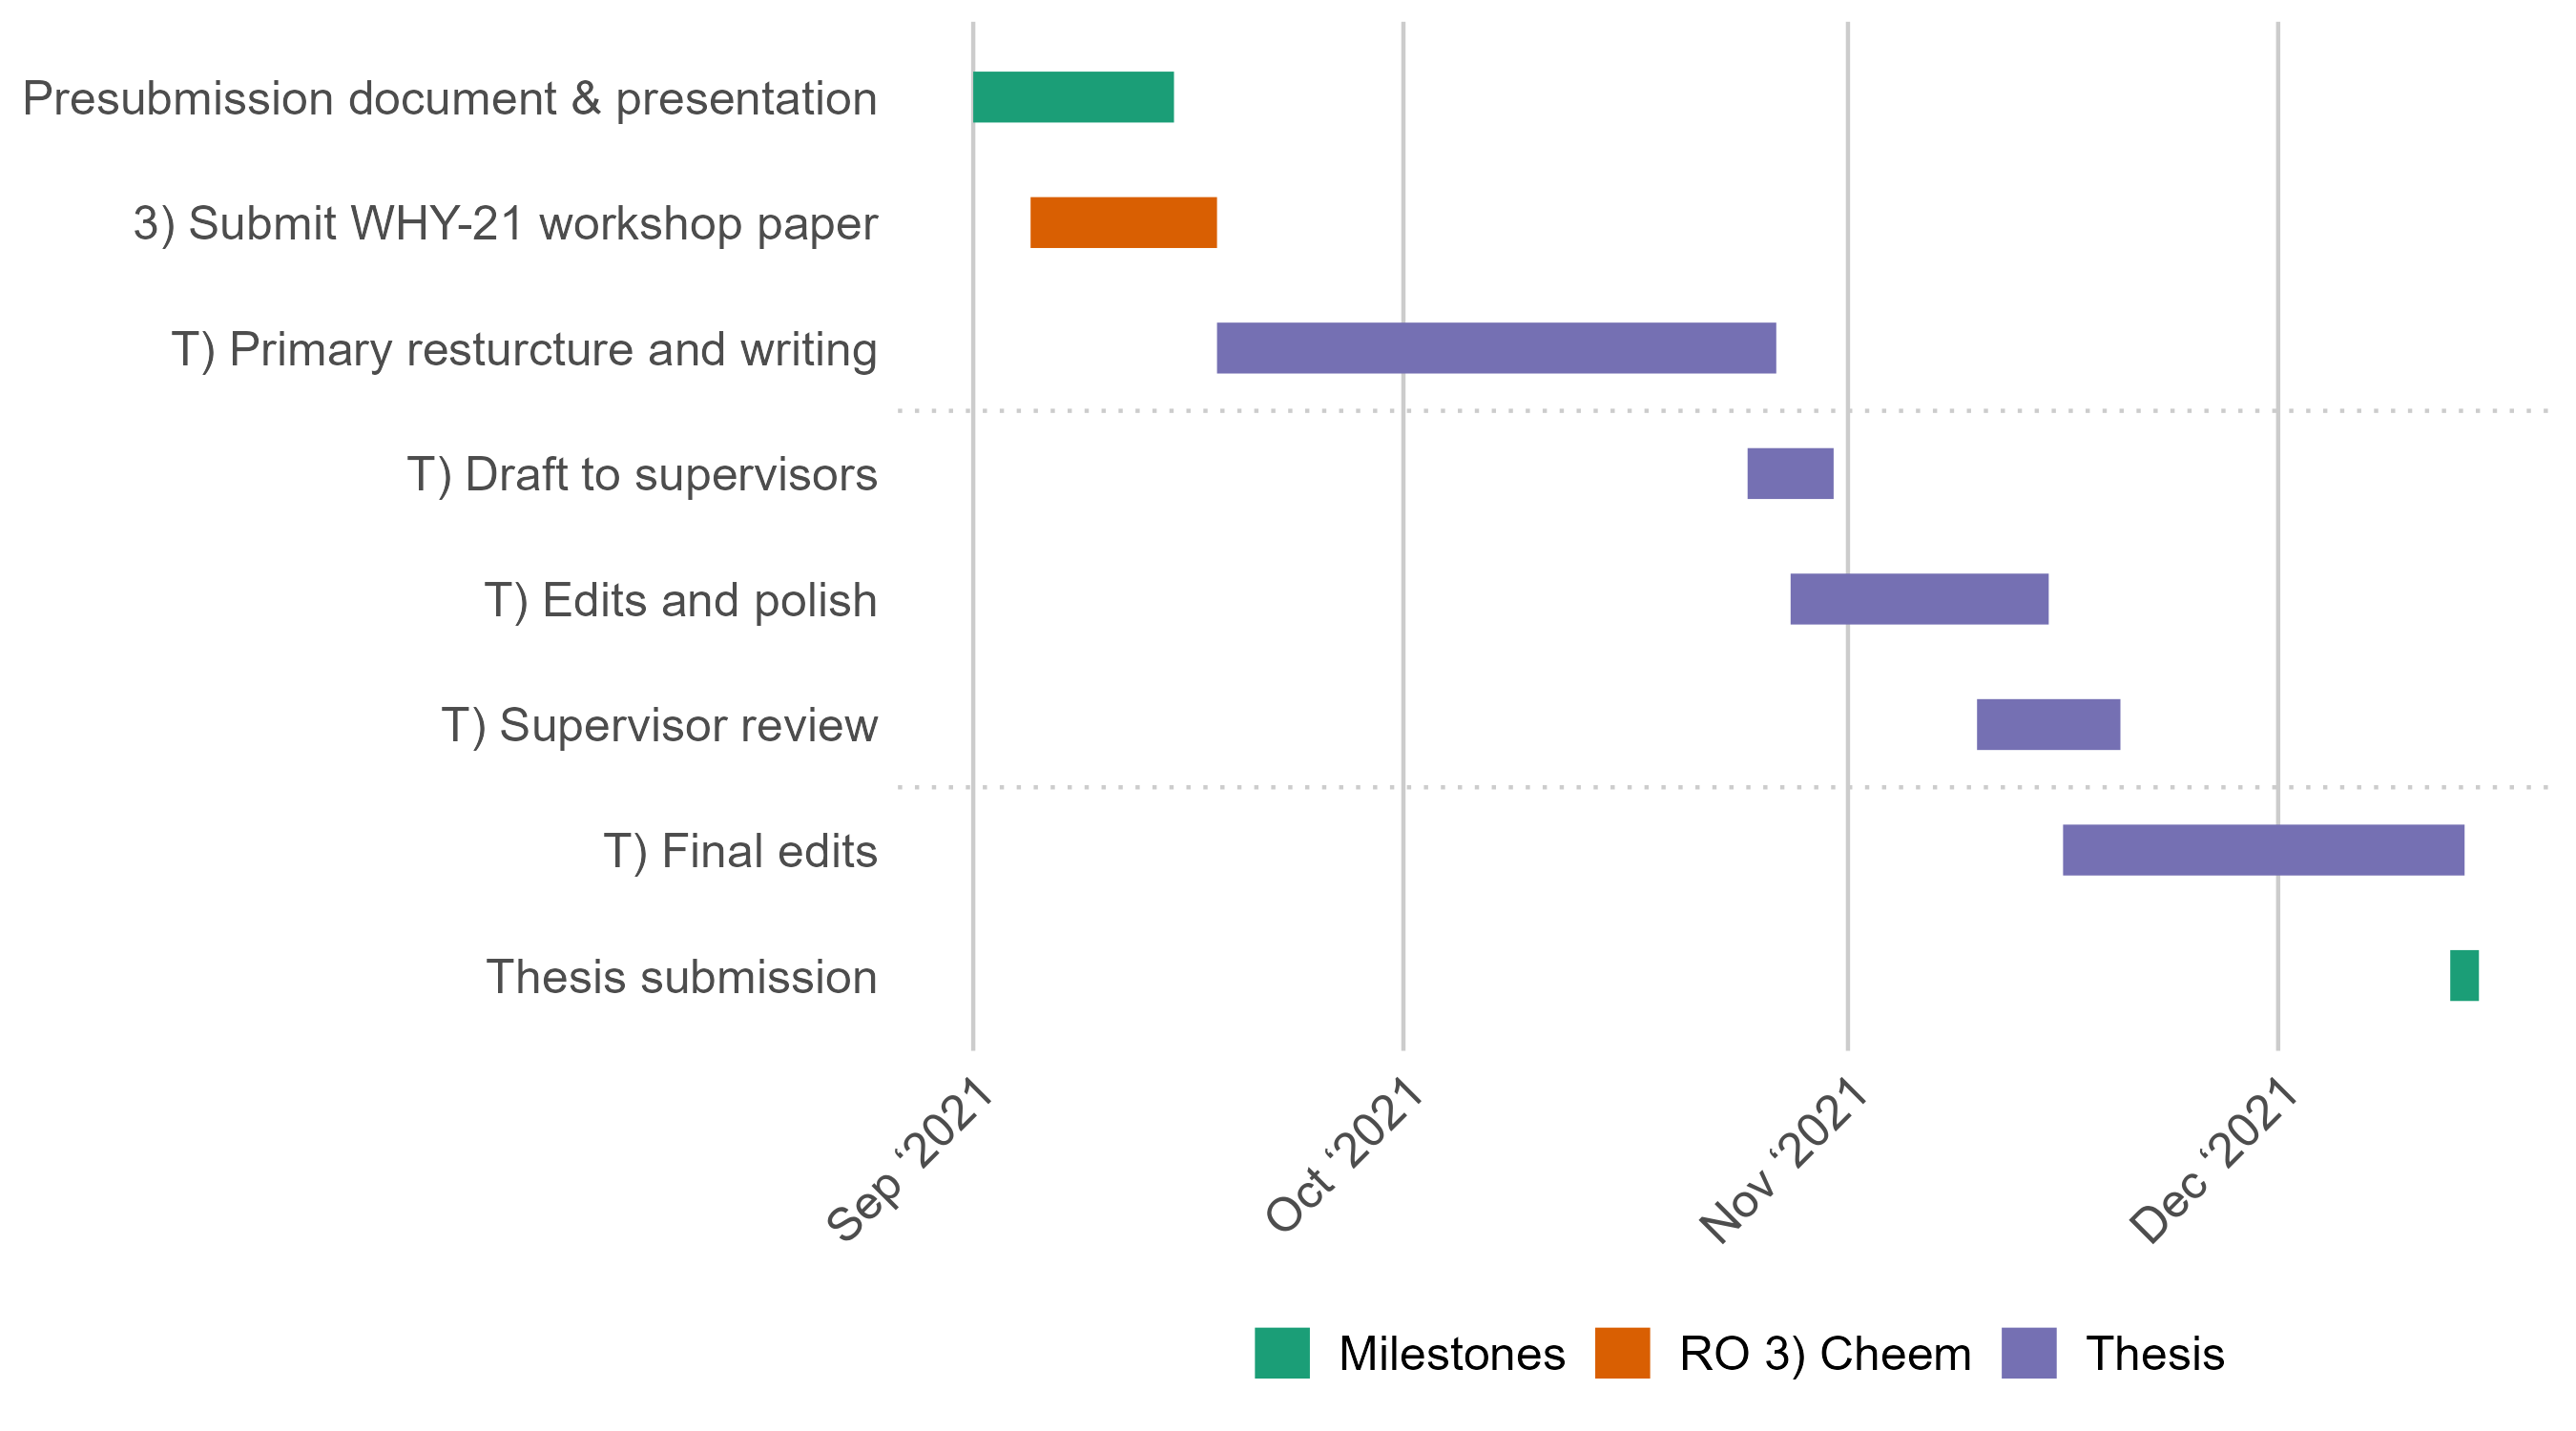
\includegraphics[width=1\linewidth,]{figures/timeline_post_presubmission} 

}

\caption{Proposed research timeline.}\label{fig:timeline}
\end{figure}

\hypertarget{adverse-conditions}{%
\subsection{Adverse conditions}\label{adverse-conditions}}

In addition to the ongoing COVID-19 pandemic, I faced major rework in the second project to accommodate physical distancing. Namely, the user study that was all but ready to be run in person, had to be restructured, to better suit crowdsourcing online. The experimental factors had to be simplified for less knowledgeable people with no interactive help or direction. The shiny apps that hosted the application were not suitably resourced to handle the volume of the crowdsourcing which further exasperated the situation.

Regular circumstances were also obstructed as I took 2 intermissions out of concern for my mental health, namely anxiety and depression, stemming from my obsessive-compulsive personality disorder.

Intermission periods:

\begin{itemize}
\tightlist
\item
  13/03/2020 - 08/05/2020
\item
  15/11/2020 - 01/10/2021
\end{itemize}

\hypertarget{other-contributions}{%
\section{Other Contributions}\label{other-contributions}}

\begin{itemize}
\tightlist
\item
  ``Is IEEE VIS \emph{that} good?'' AltVis (Spyrison, Lee, and Besançon 2021)
\item
  Student Volunteer, UseR2021 Online
\item
  A Review of the State-of-the-Art on tours Dynamic Visualization of High-dimensional Data (Lee et al. 2021)
\item
  1st place in 2020 Melbourne Data Marathon (Barrow, Chong, and Spyrison 2020)
\item
  Statistics Ph.D.~reading group, Introduction to linear \& nonlinear dimension reduction, discussing: ``Dimensionality Reduction: A Comparative
  Review. van der Maaten'' 2020
\item
  Student Volunteer, CHI Down Under 2020 Online
\item
  NUMBAT Workshop, Animating ggplot2 figures with gganimate, 2018
\item
  Student Volunteer, UseR2018 Online
\end{itemize}

\hypertarget{sec:acknowledgements}{%
\section{Acknowledgements}\label{sec:acknowledgements}}

I would like to thank Professor Przemyslaw Biecek for his time and input in suggesting to look at SHAP local explanations and try applying to the FIFA dataset.

This research was supported by an Australian government Research Training Program (RTP) scholarship. This article was created in \texttt{R} (R Core Team 2020) and \texttt{rmarkdown} (Xie, Allaire, and Grolemund 2018).

For transparency and reproducibility, the source files are made available at \href{https://github.com/nspyrison/phd_milestones}{github.com/nspyrison/phd\_milestones}.

\hypertarget{references}{%
\section*{References}\label{references}}
\addcontentsline{toc}{section}{References}

\hypertarget{refs}{}
\begin{CSLReferences}{1}{0}
\leavevmode\hypertarget{ref-adadi_peeking_2018}{}%
Adadi, Amina, and Mohammed Berrada. 2018. {``Peeking Inside the Black-Box: A Survey on Explainable Artificial Intelligence ({XAI}).''} \emph{IEEE Access} 6: 52138--60.

\leavevmode\hypertarget{ref-anscombe_graphs_1973}{}%
Anscombe, F. J. 1973. {``Graphs in Statistical Analysis.''} \emph{The American Statistician} 27 (1): 17--21. \url{https://doi.org/10.2307/2682899}.

\leavevmode\hypertarget{ref-arrieta_explainable_2020}{}%
Arrieta, Alejandro Barredo, Natalia Díaz-Rodríguez, Javier Del Ser, Adrien Bennetot, Siham Tabik, Alberto Barbado, Salvador García, Sergio Gil-López, Daniel Molina, and Richard Benjamins. 2020. {``Explainable {Artificial} {Intelligence} ({XAI}): {Concepts}, Taxonomies, Opportunities and Challenges Toward Responsible {AI}.''} \emph{Information Fusion} 58: 82--115.

\leavevmode\hypertarget{ref-asimov_grand_1985}{}%
Asimov, Daniel. 1985. {``The Grand Tour: A Tool for Viewing Multidimensional Data.''} \emph{{SIAM} Journal on Scientific and Statistical Computing} 6 (1): 128--43. https://doi.org/\url{https://doi.org/10.1137/0906011}.

\leavevmode\hypertarget{ref-barrow_melbourne_2020}{}%
Barrow, Madeleine, Jieyang Chong, and Nicholas Spyrison. 2020. {``Melbourne {Datathon} 2020.''} In \emph{Melbourne {Datathon} 2020, {Insights} Category}. \url{https://www.overleaf.com/project/5f614799515ac0000119daf7}.

\leavevmode\hypertarget{ref-biecek_dalex_2018}{}%
Biecek, Przemyslaw. 2018. {``{DALEX}: {Explainers} for {Complex} {Predictive} {Models} in {R}.''} \emph{Journal of Machine Learning Research} 19 (84): 1--5. \url{https://jmlr.org/papers/v19/18-416.html}.

\leavevmode\hypertarget{ref-biecek_explanatory_2021}{}%
Biecek, Przemyslaw, and Tomasz Burzykowski. 2021. \emph{Explanatory Model Analysis: Explore, Explain, and Examine Predictive Models}. CRC Press.

\leavevmode\hypertarget{ref-cook_manual_1997}{}%
Cook, Dianne, and Andreas Buja. 1997. {``Manual Controls for High-Dimensional Data Projections.''} \emph{Journal of Computational and Graphical Statistics} 6 (4): 464--80. \url{https://doi.org/10.2307/1390747}.

\leavevmode\hypertarget{ref-cook_grand_2008}{}%
Cook, Dianne, Andreas Buja, Eun-Kyung Lee, and Hadley Wickham. 2008. {``Grand Tours, Projection Pursuit Guided Tours, and Manual Controls.''} In \emph{Handbook of Data Visualization}, 295--314. Berlin, Heidelberg: Springer Berlin Heidelberg. \url{https://doi.org/10.1007/978-3-540-33037-0_13}.

\leavevmode\hypertarget{ref-lee_review_2021}{}%
Lee, Stuart, Dianne Cook, Natalia da Silva, Ursula Laa, Earo Wang, Nick Spyrison, and H. Sherry Zhang. 2021. {``A {Review} of the {State}-of-the-{Art} on {Tours} for {Dynamic} {Visualization} of {High}-{Dimensional} {Data}.''} \emph{arXiv:2104.08016 {[}Cs, Stat{]}}, April. \url{http://arxiv.org/abs/2104.08016}.

\leavevmode\hypertarget{ref-leone_fifa_2020}{}%
Leone, Stefano. 2020. {``{FIFA} 20 Complete Player Dataset.''} \url{https://kaggle.com/stefanoleone992/fifa-20-complete-player-dataset}.

\leavevmode\hypertarget{ref-lundberg_unified_2017}{}%
Lundberg, Scott, and Su-In Lee. 2017. {``A Unified Approach to Interpreting Model Predictions.''} \emph{arXiv Preprint arXiv:1705.07874}.

\leavevmode\hypertarget{ref-matejka_same_2017}{}%
Matejka, Justin, and George Fitzmaurice. 2017. {``Same Stats, Different Graphs: Generating Datasets with Varied Appearance and Identical Statistics Through Simulated Annealing.''} In \emph{Proceedings of the 2017 {CHI} Conference on Human Factors in Computing Systems - {CHI} '17}, 1290--94. Denver, Colorado, {USA}: {ACM} Press. \url{https://doi.org/10.1145/3025453.3025912}.

\leavevmode\hypertarget{ref-pearson_liii._1901}{}%
Pearson, Karl. 1901. {``{LIII}. On Lines and Planes of Closest Fit to Systems of Points in Space.''} \emph{The London, Edinburgh, and Dublin Philosophical Magazine and Journal of Science} 2 (11): 559--72.

\leavevmode\hypertarget{ref-r_core_team_r:_2020}{}%
R Core Team. 2020. \emph{R: {A} {Language} and {Environment} for {Statistical} {Computing}}. Vienna, Austria: R Foundation for Statistical Computing. \url{https://www.R-project.org/}.

\leavevmode\hypertarget{ref-ribeiro_why_2016}{}%
Ribeiro, Marco Tulio, Sameer Singh, and Carlos Guestrin. 2016. {``"{Why} {Should} {I} {Trust} {You}?": {Explaining} the {Predictions} of {Any} {Classifier}.''} \emph{arXiv:1602.04938 {[}Cs, Stat{]}}, February. \url{http://arxiv.org/abs/1602.04938}.

\leavevmode\hypertarget{ref-spyrison_spinifex_2020}{}%
Spyrison, Nicholas, and Dianne Cook. 2020. {``Spinifex: An r Package for Creating a Manual Tour of Low-Dimensional Projections of Multivariate Data.''} \emph{The R Journal} 12 (1): (accepted).

\leavevmode\hypertarget{ref-spyrison_is_2021}{}%
Spyrison, Nicholas, Benjamin Lee, and Lonni Besançon. 2021. {``"{Is} {IEEE} {VIS} *That* Good?" {On} Key Factors in the Initial Assessment of Manuscript and Venue Quality.''} \emph{OSF Preprints}, July. \url{https://doi.org/10.31219/osf.io/65wm7}.

\leavevmode\hypertarget{ref-tukey_exploratory_1977}{}%
Tukey, John W. 1977. \emph{Exploratory Data Analysis}. Vol. 32. Pearson.

\leavevmode\hypertarget{ref-xie_r_2018}{}%
Xie, Yihui, J. J. Allaire, and Garrett Grolemund. 2018. \emph{R Markdown: The Definitive Guide}. Boca Raton, Florida: Chapman; Hall/{CRC}. \url{https://bookdown.org/yihui/rmarkdown}.

\end{CSLReferences}

\end{document}
